\chapter{Giãn nở Friedmann, bức xạ và vật chất tối}

\section{Ôn lại phương trình vũ trụ học cơ bản}

Ở những thang lớn hơn các cụm thiên hà, vũ trụ được coi là đồng nhất. Chọn tọa độ sao cho ta ở tại \(x=0\), và đặt một thiên hà điển hình, hoặc đơn giản là một hạt tưởng tượng chuyển động theo dòng Hubble, tại \(x=1\). Khi đó khoảng cách vật lý từ nó đến ta, theo định nghĩa, chính là thừa số tỉ lệ \(a(t)\). Một điểm tại \(x=2\) cách ta \(2a(t)\), và cứ thế tiếp tục.

\begin{figure}[ht]
\centering
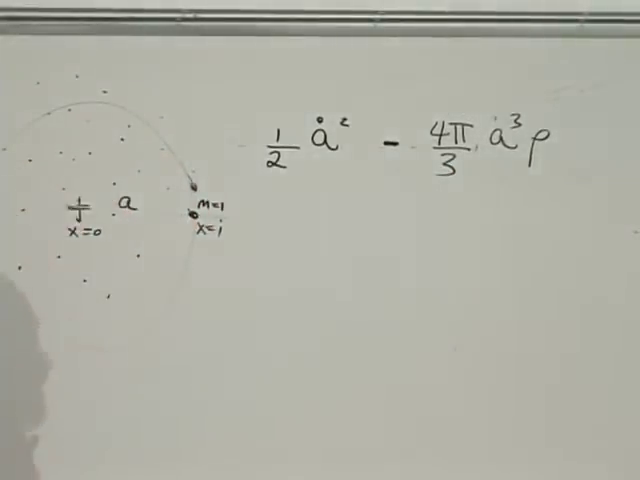
\includegraphics[width=0.78\textwidth]{lecture_03_figure_02.png}
\caption{Hình cầu đồng nhất tâm tại \(x=0\), một thiên hà đồng chuyển động tại \(x=1\), và cân bằng năng lượng Newton cho \(a(t)\).}
\end{figure}

Chỉ vật chất nằm bên trong hình cầu bán kính \(a(t)\) mới góp phần vào lực hút hấp dẫn tác dụng lên hạt tại \(x=1\). Gán cho hạt đó khối lượng đơn vị. Động năng của nó là
\begin{equation}
\frac{1}{2}\dot a^2.
\end{equation}
Khối lượng chứa trong hình cầu là
\begin{equation}
M_{\mathrm{enc}}=\frac{4\pi}{3}a^3\rho,
\end{equation}
nên thế năng hấp dẫn là
\begin{equation}
-\frac{G M_{\mathrm{enc}}}{a}
=
-\frac{4\pi G}{3}a^2\rho.
\end{equation}
\editorialnote{Tại mốc thời gian bài giảng 00:05:30, trên bảng hiển thị rõ hạng động năng và hạng thế năng phụ thuộc vào mật độ. Hệ số đầy đủ được viết ở đây suy ra từ phần diễn giải bằng lời.}

Bảo toàn năng lượng cho
\begin{equation}
\frac{1}{2}\dot a^2-\frac{4\pi G}{3}a^2\rho=\text{const}.
\end{equation}
Khi đó hằng số được viết là \(-k\), với lưu ý quen thuộc rằng phép chuẩn hóa tiêu chuẩn thực ra chỉ cố định ký hiệu ấy sau khi nhân phương trình với \(2\). Ở dạng tiêu chuẩn,
\begin{equation}
\dot a^2=\frac{8\pi G}{3}a^2\rho-k,
\end{equation}
và chia cho \(a^2\) cho
\begin{equation}
\left(\frac{\dot a}{a}\right)^2=\frac{8\pi G}{3}\rho-\frac{k}{a^2}.
\end{equation}
Đây là phương trình Friedmann ở dạng được dùng xuyên suốt phần thảo luận.

\begin{figure}[ht]
\centering
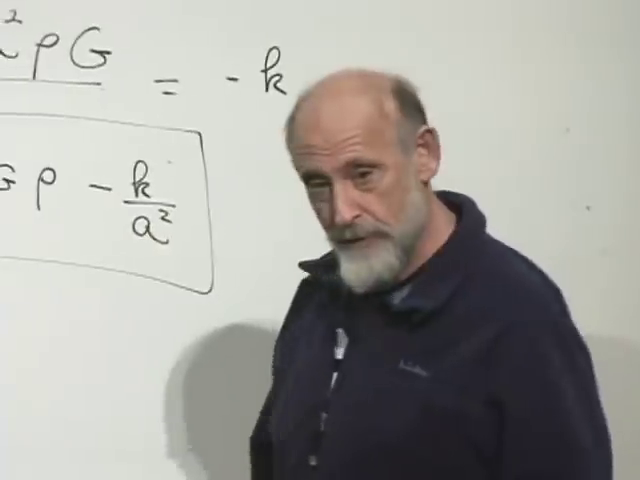
\includegraphics[width=0.56\textwidth]{lecture_03_figure_03.png}
\caption{Phần đóng góp độ cong \(-k/a^2\) được tách riêng trong phương trình Friedmann.}
\end{figure}

Về mặt thực nghiệm, hạng độ cong rất gần bằng 0, đủ gần để ở mức này việc đơn giản bỏ qua nó là một gần đúng rất tốt. Nó quả thực tương ứng với độ cong của không gian, nhưng về quan sát thì ở đây nó quá nhỏ đến mức không thể xác định ngay cả dấu của nó.

Phương trình ấy cũng xuất phát từ thuyết tương đối rộng. Ở dạng sơ đồ, phương trình Einstein thành phần thời-gian thời-gian là
\begin{equation}
R_{00}-\frac{1}{2}g_{00}R \propto T_{00}.
\end{equation}
\editorialnote{Phần thảo luận ở đây chỉ nêu cấu trúc tensor, không nêu hệ số số học tổng thể chính xác.}
Với một metric đồng nhất đang giãn nở, vế hình học sinh ra tổ hợp của \(\dot a/a\) và \(k/a^2\), còn vế vật chất sinh ra mật độ năng lượng. Ở giai đoạn này, lập luận Newton và phương trình Einstein đang nói cùng một điều.

Điều đó cũng làm thay đổi ý nghĩa của \(\rho\). Từ đây trở đi, tốt hơn nên gọi \(\rho\) là mật độ năng lượng. Với vật chất chuyển động chậm trong hệ đồng chuyển động, đó đơn giản là mật độ năng lượng nghỉ.

\section{Thời kỳ vật chất chi phối}

Bây giờ giả sử mật độ năng lượng do vật chất đứng yên trong hệ đồng chuyển động mang. Xét một hình lập phương có cạnh dài một đơn vị tọa độ. Các cạnh vật lý của nó đều là \(a(t)\), nên thể tích vật lý của nó là \(a^3(t)\). Nếu khối lượng-năng lượng bên trong khối lập phương đồng chuyển động đó là \(M\), và vật chất chuyển động theo dòng thay vì đi qua biên, thì
\begin{equation}
\rho_m=\frac{M}{a^3}.
\end{equation}

Đây là trường hợp vật chất chi phối. Trong lý tưởng hóa này, các hạt đứng yên trong hộp, nên nhiệt độ được coi bằng 0 và áp suất được coi bằng 0. Áp suất sẽ đòi hỏi các hạt đi qua biên của hộp.

Với \(k\approx 0\), phương trình trở thành
\begin{equation}
\left(\frac{\dot a}{a}\right)^2=\frac{8\pi G}{3}\frac{M}{a^3}.
\end{equation}
Hãy thử một luật lũy thừa,
\begin{equation}
a(t)=Ct^p.
\end{equation}
Khi đó
\begin{equation}
\frac{\dot a}{a}=\frac{p}{t},
\end{equation}
nên vế trái biến thiên như \(t^{-2}\), còn vế phải biến thiên như \(t^{-3p}\). Khớp số mũ cho ta
\begin{equation}
3p=2,
\qquad
p=\frac{2}{3}.
\end{equation}
Do đó
\begin{equation}
a(t)\propto t^{2/3}.
\end{equation}
Giữ lại hệ số thì được
\begin{equation}
C^3=6\pi G M.
\end{equation}

Điểm mấu chốt của nghiệm này là luật lũy thừa. Một vũ trụ do vật chất chi phối giãn nở theo lũy thừa hai phần ba của thời gian, không phải tuyến tính. Định luật này mô tả một thời kỳ trung gian dài, từ khoảng \(10^5\) năm sau Vụ Nổ Lớn đến vài tỷ năm sau đó. Vũ trụ hiện nay không đúng nghĩa là do vật chất chi phối, vì năng lượng tối hiện chi phối, nhưng vật chất thông thường cũng như một quãng dài của lịch sử vũ trụ được mô tả theo cách này.

\section{Thời kỳ bức xạ chi phối}

Trước đó, mật độ năng lượng do bức xạ chi phối. Lý do rất đơn giản. Vũ trụ chứa một số lượng photon khổng lồ, xấp xỉ \(10^9\) photon cho mỗi proton, và khi vũ trụ bị nén lại thì năng lượng của các photon ấy tăng lên.

Photon không có khối lượng nghỉ, nhưng nó có năng lượng. Năng lượng của nó là
\begin{equation}
E_\gamma=h\nu=\frac{hc}{\lambda}.
\end{equation}
Giả thiết then chốt là khi vũ trụ giãn nở, bước sóng photon giãn theo nó:
\begin{equation}
\lambda\propto a.
\end{equation}
Một sóng trong hộp cho ta bức tranh đúng. Nếu hộp lớn lên, bước sóng của mode tăng theo hộp. Cùng ý tưởng đó được dùng ở đây cho vũ trụ đang giãn nở.

Vì \(\lambda\propto a\), năng lượng của mỗi photon biến thiên như
\begin{equation}
E_\gamma\propto a^{-1}.
\end{equation}
Lại xét một hộp đơn vị đồng chuyển động. Photon đi vào rồi đi ra, nhưng trung bình thì số lượng bên trong vẫn giữ cố định. Khi đó tổng năng lượng photon trong hộp cũng biến thiên như \(a^{-1}\). Chia cho thể tích vật lý \(a^3\), mật độ năng lượng bức xạ biến thiên như
\begin{equation}
\rho_r\propto a^{-4}.
\end{equation}

Chính nhân tử phụ thêm \(a^{-1}\) đó tạo nên toàn bộ khác biệt. Vật chất bị pha loãng vì vũ trụ giãn nở. Bức xạ bị pha loãng vì lý do ấy, và còn vì mỗi photon đều bị dịch đỏ.

Do đó, phương trình Friedmann cho một vũ trụ do bức xạ chi phối là
\begin{equation}
\left(\frac{\dot a}{a}\right)^2=\frac{8\pi G}{3}\frac{M_r}{a^4}.
\end{equation}
\editorialnote{Phần trình bày bằng lời dùng lại ký hiệu \(M\) cho hằng số mới này. Chỉ số dưới \(r\) được thêm vào ở đây chỉ để tránh nhầm lẫn với trường hợp vật chất.}

Dùng cùng dạng thử \(a(t)=Ct^p\). Vế trái lại biến thiên như \(t^{-2}\), còn vế phải biến thiên như \(t^{-4p}\). Khớp số mũ cho ta
\begin{equation}
4p=2,
\qquad
p=\frac{1}{2}.
\end{equation}
Vì vậy
\begin{equation}
a(t)\propto t^{1/2}.
\end{equation}
Giữ lại hệ số thì được
\begin{equation}
C^4=\frac{32\pi G}{3}M_r.
\end{equation}

\begin{classroomqa}
\lecturetimestamp{00:35:41}
\audiencequestion{Tại sao trong đó lại có \(G\)?}
\lecturerresponse{Bởi vì cái gây hấp dẫn là mật độ năng lượng, không phải chỉ riêng khối lượng nghỉ. Đối với vật chất chuyển động chậm, sự khác biệt này dễ bị bỏ qua, nhưng photon buộc ta phải đối mặt với nó: chúng không có khối lượng nghỉ mà vẫn gây hấp dẫn.}
\end{classroomqa}

Một hộp đầy bức xạ làm cho điểm này trở nên cụ thể. Hãy đẩy một cái hộp chứa đầy photon. Khi hộp gia tốc, thành chuyển động về phía các photon bị chúng va mạnh hơn thành chuyển động ra xa chúng, nên ta phải đẩy mạnh hơn để chống lại áp suất bức xạ. Vì vậy hộp có thêm quán tính, và theo nguyên lý tương đương, phần quán tính tăng thêm đó cũng có nghĩa là có thêm khối lượng hấp dẫn. Đây là lập luận cái hộp photon được dùng ở đây để nói rằng năng lượng gây hấp dẫn.

\begin{classroomqa}
\lecturetimestamp{00:38:11}
\audiencequestion{Có phương trình nào trong hai phương trình này có nghiệm với \(a\) giảm theo thời gian không?}
\lecturerresponse{Có. Nếu khôi phục hạng độ cong \(k/a^2\), sẽ có những nghiệm giãn nở rồi co lại. Đó không có vẻ là điều vũ trụ của chúng ta đang làm, nhưng phương trình cho phép như vậy.}
\end{classroomqa}

\begin{classroomqa}
\lecturetimestamp{00:38:44}
\audiencequestion{Còn bảo toàn năng lượng thì sao?}
\lecturerresponse{Nếu khôi phục hạng \(k\) và nhân phương trình trở lại với \(a^2\), thì phương trình vũ trụ học chính là định luật bảo toàn. Vật chất hay bức xạ ở một vế chỉ là một phần của việc hạch toán. Sự giãn nở đóng góp phần động năng và phần hấp dẫn, và cân bằng tổng thể được bảo toàn.}
\end{classroomqa}

\section{Vật chất và bức xạ cùng hiện diện}

Vũ trụ học thực tế có cả vật chất lẫn bức xạ. Mật độ của chúng biến thiên khác nhau:
\begin{equation}
\rho_m\propto a^{-3},
\qquad
\rho_r\propto a^{-4}.
\end{equation}
Vì thế với \(a\) nhỏ, bức xạ chi phối. Với \(a\) lớn, vật chất chi phối. Lần ngược về quá khứ, do đó vũ trụ sơ khai hẳn phải do bức xạ chi phối.

\begin{figure}[ht]
\centering
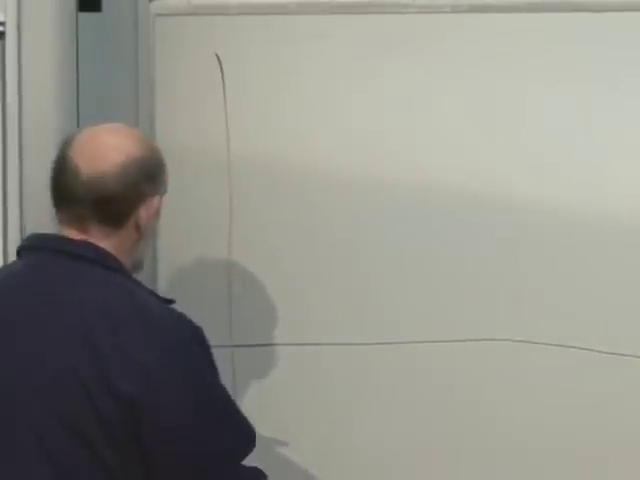
\includegraphics[width=0.68\textwidth]{lecture_03_figure_05.png}
\caption{Các trục để so sánh mật độ năng lượng của vật chất và bức xạ theo thừa số tỉ lệ.}
\end{figure}

\editorialnote{Tại mốc thời gian bài giảng 00:44:45, trên bảng lúc bắt đầu đồ thị so sánh chỉ có các trục. Các đường cong vật chất và bức xạ được thảo luận ngay sau đó được mô tả trong văn bản thay vì vẽ lại ở đây.}

Đường cong vật chất giảm như \(a^{-3}\). Đường cong bức xạ giảm như \(a^{-4}\). Cả hai đều phân kỳ khi \(a\to 0\), nhưng đường cong bức xạ tăng nhanh hơn ở đó, nên hai đường cắt nhau tại một thừa số tỉ lệ cân bằng. Một ước lượng thô đặt sự chuyển tiếp này sau khoảng \(10^4\) năm, có lẽ hơi nhiều hơn một chút.

Ý đó cũng có thể được biểu diễn trên đồ thị \(a(t)\) theo \(t\). Ban đầu, sự giãn nở có dạng \(t^{1/2}\). Về sau, nó có dạng \(t^{2/3}\). Sự thay đổi không phải là một bước nhảy; đó là một chuyển tiếp liên tục qua một khoảng thời gian tương đối hẹp.

\begin{classroomqa}
\lecturetimestamp{00:44:04}
\audiencequestion{Khi vũ trụ già đi, số mũ \(p\) có biến đổi liên tục từ \(1/2\) đến \(2/3\) không?}
\lecturerresponse{Có. Nó không nhảy bậc. Sự thay đổi là liên tục, dù diễn ra trong một khoảng thời gian khá hẹp.}
\end{classroomqa}

\section{Nhiệt độ, tái hợp và tán xạ lần cuối}

Đại lượng tiếp theo là nhiệt độ. Nếu năng lượng của một photon điển hình tỉ lệ như \(a^{-1}\), thì nhiệt độ của nền bức xạ cũng vậy:
\begin{equation}
T\propto a^{-1}.
\end{equation}
Nếu \(a\) tăng gấp đôi, thì nhiệt độ giảm còn một nửa.

Lấy nhiệt độ photon hiện nay vào khoảng \(3\,\mathrm K\), và nhiệt độ ion hóa vào khoảng \(3000\,\mathrm K\), xấp xỉ nhiệt độ bề mặt Mặt Trời. Khi đó
\begin{equation}
\frac{a_{\mathrm{today}}}{a_{\mathrm{ion}}}\sim 10^3.
\end{equation}
Dùng định luật của giai đoạn muộn do vật chất chi phối \(a\propto t^{2/3}\),
\begin{equation}
\left(\frac{t_{\mathrm{today}}}{t_{\mathrm{ion}}}\right)^{2/3}\sim 10^3,
\end{equation}
nên
\begin{equation}
\frac{t_{\mathrm{today}}}{t_{\mathrm{ion}}}\sim 1000^{3/2}\sim 3\times 10^4.
\end{equation}
Lấy tuổi của vũ trụ, ở mức gần đúng này, là \(10^{10}\) năm, ta được
\begin{equation}
t_{\mathrm{ion}}\sim 3\times 10^5\ \mathrm{years}.
\end{equation}

Đây là thời kỳ khi hydrogen và helium thôi không còn bị ion hóa hoàn toàn. Trước đó, vũ trụ là một plasma nóng. Vì sao plasma lại mờ đục? Vì các điện tích tự do đáp ứng rất mạnh với sóng điện từ. Điện trường làm các điện tích dao động qua lại, môi trường hành xử như một chất dẫn điện, mà các chất dẫn điện thì mờ đục. Đó là phép tương tự thích hợp với bề mặt Mặt Trời.

Khi vũ trụ nguội đi đủ để các electron tái kết hợp với các hạt nhân, các nguyên tử trung hòa thông thường hình thành và vũ trụ trở nên trong suốt hơn nhiều. Sự chuyển tiếp này không sắc nét vô hạn. Nó là một vùng mờ, hay một khoảng thời gian mờ, nhưng đối với vũ trụ học thì đủ sắc nét để được gọi là mặt tán xạ cuối cùng.

Nhìn ra xa có nghĩa là nhìn ngược về quá khứ. Các thiên hà ở gần cho thấy quá khứ gần đây. Các thiên hà xa hơn cho thấy những thời điểm sớm hơn. Nhìn đủ xa, mọi đường ngắm đều chạm tới thời kỳ khi vũ trụ vẫn còn bị ion hóa và mờ đục. Bức xạ điện từ không thể cho thấy bất cứ điều gì sớm hơn thời kỳ đó.

Về nguyên tắc, những sứ giả khác có thể thăm dò các thời điểm sớm hơn. Neutrino trung hòa điện và sẽ tách ra sớm hơn. Graviton, nếu con người có thể quan sát được chúng, sẽ đến từ những thời kỳ còn sớm hơn nữa. Nhưng chính sự yếu của tương tác cho phép chúng đi xuyên qua plasma sơ khai cũng khiến chúng cực kỳ khó phát hiện.

Nếu vũ trụ từng nóng như bề mặt Mặt Trời theo mọi hướng, thì vì sao bầu trời không sáng chói đến lóa mắt? Bởi vì mặt tán xạ cuối cùng đang lùi ra xa, và các photon đến từ đó đã bị dịch đỏ bởi xấp xỉ cùng hệ số \(10^3\), hệ số phân cách \(3000\,\mathrm K\) với \(3\,\mathrm K\). Thứ đến với chúng ta là bức xạ vi ba, chứ không phải ánh sáng Mặt Trời nhìn thấy được.

\begin{classroomqa}
\lecturetimestamp{01:03:51}
\audiencequestion{Vậy các kính thiên văn của chúng ta không thể nhìn về thời điểm sớm hơn khoảng \(300{,}000\) năm sao?}
\lecturerresponse{Kính thiên văn điện từ thì không thể. Trước thời điểm đó, vũ trụ bị ion hóa và mờ đục. Ít nhất về nguyên tắc, những sứ giả khác có thể thăm dò các thời kỳ sớm hơn.}
\end{classroomqa}

\begin{classroomqa}
\lecturetimestamp{01:08:43}
\audiencequestion{Khi thầy nói đến nhiệt độ của một photon, ý thầy là nhiệt độ của một vật đen có đỉnh bức xạ đó. Nhưng đại lượng ấy không tuyến tính theo bước sóng, đúng không?}
\lecturerresponse{Đúng. Nhiệt độ về cơ bản là năng lượng của một photon điển hình, nên đối với photon nó tỉ lệ nghịch với bước sóng. Định luật \(T^4\) nói về mật độ năng lượng, không phải năng lượng của một photon đơn lẻ. Nó kết hợp năng lượng trên mỗi photon với số photon trên một đơn vị thể tích, và mật độ số tỉ lệ như \(T^3\).}
\end{classroomqa}

Do đó
\begin{equation}
n_\gamma\propto T^3,
\qquad
\rho_\gamma\propto T^4.
\end{equation}

\section{Vật chất tối từ các đường cong quay}

Vật chất tối xuất hiện thông qua các đường cong quay của thiên hà. Nó không được suy ra từ phương trình Friedmann ở quy mô lớn, mà từ thiên văn học ở quy mô thiên hà.

Bắt đầu với bài toán Newton đơn giản nhất: một vật nhẹ khối lượng \(m\) quay quanh một khối lượng trung tâm \(M\) ở bán kính \(r\). Lực hấp dẫn là
\begin{equation}
\frac{GMm}{r^2},
\end{equation}
và gia tốc hướng tâm là \(v^2/r\). Định luật Newton cho
\begin{equation}
m\frac{v^2}{r}=\frac{GMm}{r^2}.
\end{equation}
Khử \(m\), nhân với \(r\), và thu được
\begin{equation}
v(r)=\sqrt{\frac{GM}{r}}.
\end{equation}
Vì vậy, nếu khối lượng gây hấp dẫn tập trung gần tâm, thì tốc độ quỹ đạo giảm như \(r^{-1/2}\).

Đó là điều người ta sẽ kỳ vọng nếu khối lượng phân bố theo ánh sáng. Phần lớn vật chất nhìn thấy được trong một thiên hà nằm gần lõi, nên khi đó các ngôi sao ở ngoài sẽ hành xử rất giống các hành tinh ở phần ngoài của Hệ Mặt Trời. Các nhà thiên văn suy ra các tốc độ quỹ đạo bằng cách đo chênh lệch dịch chuyển Doppler qua một thiên hà ở gần, so sánh phía chuyển động về phía chúng ta với phía chuyển động ra xa chúng ta sau khi đã trừ đi chuyển động lùi ra xa tổng thể của cả thiên hà. Các tốc độ quỹ đạo đo được vẫn gần như không đổi ra tới các bán kính lớn.

Vậy hãy thay khối lượng trung tâm \(M\) bằng khối lượng bao trong \(M(r)\):
\begin{equation}
\frac{v^2}{r}=\frac{G M(r)}{r^2}.
\end{equation}
Nếu \(v(r)\) xấp xỉ không đổi, thì
\begin{equation}
M(r)\propto r.
\end{equation}
Nói cách khác, khối lượng gây hấp dẫn tiếp tục tăng theo bán kính ngay cả ở những nơi mà ánh sáng nhìn thấy được thì không.

Bây giờ giả sử, như phần thảo luận làm để đơn giản hóa, rằng phân bố khối lượng gần như đối xứng cầu. Khi đó
\begin{equation}
M(R)=\int_0^R 4\pi r^2\rho(r)\,dr.
\end{equation}
Nếu \(M(R)\propto R\), thì lấy đạo hàm theo \(R\) cho
\begin{equation}
4\pi R^2\rho(R)\propto 1,
\end{equation}
và do đó
\begin{equation}
\rho(r)\propto \frac{1}{r^2}.
\end{equation}

\begin{classroomqa}
\lecturetimestamp{01:28:18}
\audiencequestion{Có vẻ như mật độ phải biến thiên như \(1/r^2\). Có lý do nào cho điều đó không?}
\lecturerresponse{Từ đường cong quay phẳng quan sát được, người ta suy ra \(M(R)\propto R\), rồi lấy đạo hàm thì được \(\rho(r)\propto 1/r^2\). Ngoài điều đó ra, ở đây không nêu ra một lời giải thích đơn giản nào từ các nguyên lý đầu tiên; các mô phỏng chi tiết đảm nhiệm phần lớn công việc.}
\end{classroomqa}

Kết luận vững chắc là một thiên hà chứa nhiều khối lượng gây hấp dẫn hơn rất nhiều so với điều chỉ riêng vật chất phát sáng gợi ra, cỡ lớn hơn vài lần và, trong ước tính dùng ở đây, xấp xỉ lớn hơn một bậc độ lớn. Thiên hà nhìn thấy được nằm bên trong một quầng tối lớn hơn nhiều.

Điều gì ngăn khí thông thường duy trì một trạng thái loãng như vậy? Sự tiêu tán. Một đám mây khí co lại vì va chạm, các quá trình giống ma sát, và bức xạ cho phép nó mất năng lượng. Vật chất tối hiển nhiên không bức xạ đáng kể và hầu như không va chạm. Hấp dẫn có thể kéo nó vào trong và biến thế năng thành động năng, nhưng nếu không có sự tiêu tán hiệu quả thì nó không suy sụp thành các cấu trúc sáng đặc mà vật chất thông thường tạo thành. Thứ giữ cho quầng ấy trải rộng là động năng.

Sau đó, một số khả năng thay thế được thảo luận một cách thận trọng. Neutrino được cho là chuyển động quá nhanh để hành xử theo cách này trên các quy mô thiên hà. Một quầng làm từ hydrogen thông thường sẽ làm xáo trộn nghiêm trọng sự tổng hợp hạt nhân ở vũ trụ sơ khai. Các lỗ đen làm từ vật chất thông thường cũng được nhắc đến như những khả năng có vấn đề, vì chúng sẽ hàm ý có quá nhiều vật chất thông thường trong vũ trụ sơ khai và sẽ đặt ra các vấn đề về thấu kính hấp dẫn; phần thảo luận ở đây không khẳng định gì hơn thế.

Quầng không được mô tả như một vỏ mỏng hay một hình xuyến. Nó là một khối gần như hình cầu, không đồng nhất, có mật độ lớn hơn về phía tâm và giảm dần ra ngoài.

\begin{classroomqa}
\lecturetimestamp{01:53:12}
\audiencequestion{Thầy đang nói về Bullet Cluster phải không?}
\lecturerresponse{Vâng. Khí quan sát được trong tia X cho thấy vật chất thông thường, còn thấu kính hấp dẫn cho thấy tổng khối lượng gây hấp dẫn. Trong vụ va chạm ấy, hai phân bố đó tách rời nhau. Đó là bằng chứng mạnh mẽ cho vật chất tối thực sự, chứ không phải chỉ là một sự sửa đổi của hấp dẫn gắn riêng với vật chất nhìn thấy được.}
\end{classroomqa}

Đó là điểm quan sát cuối cùng. Về chi tiết, người ta biết rất ít về việc vật chất tối là gì, nhưng không có gì ở đây đòi hỏi một nguyên lý mới mang tính triệt để. Khả năng bảo thủ đơn giản chỉ là tự nhiên chứa thêm những hạt tương tác yếu mà cho đến nay vẫn chưa được nhận diện.
